\documentclass[12pt]{article}

\usepackage[a4paper,left=25mm,right=25mm,top=35mm,bottom=25mm]{geometry}
\usepackage{ngerman}
\usepackage{parskip}
\usepackage{times}
\usepackage{graphicx}
\usepackage{listings}
\usepackage{fancyhdr}
\usepackage{float}
\usepackage{amsmath}

\setlength{\headheight}{15.2pt}
\pagestyle{fancy}

\lhead{Bildverarbeitung und Mustererkennung\\Praktikum Blatt 4}
\rhead{Patrick Hüntelmann\\13.05.2022}

\lstset{
  basicstyle=\ttfamily,
  breakatwhitespace=false,         % sets if automatic breaks should only happen at whitespace
  breaklines=true,                 % sets automatic line breaking
  captionpos=b,                    % sets the caption-position to bottom
  deletekeywords={...},            % if you want to delete keywords from the given language
  escapeinside={\%*}{*)},          % if you want to add LaTeX within your code
  extendedchars=true,              % lets you use non-ASCII characters; for 8-bits encodings only, does not work with UTF-8
  frame=single,	                   % adds a frame around the code
  keepspaces=true,                 % keeps spaces in text, useful for keeping indentation of code (possibly needs columns=flexible)
  language=python,                 % the language of the code
  showstringspaces=false,          % underline spaces within strings only
  showtabs=false,                  % show tabs within strings adding particular underscores
  tabsize=2,	                   % sets default tabsize to 2 spaces
}

\begin{document}

\pagenumbering{arabic}

\section*{Aufgabe 4}
\subsection*{a) Glättung mit Gaußfilter}
Der erste Schritt des Canny-Kantendetektors ist eine Glättung mit einem Gaußfilter.
Hierzu wurde die Funktion \textbf{generate\_gauss\_mask} (main.py Zeile 19) implementiert, welche die Parameter $\sigma$ und \textbf{n} übergeben bekommt und mithilfe der Normalverteilung eine Maske der Größe $(2 * n + 1)^2$ berechnet.

Anschließend wird diese Maske mit der OpenCV-Funktion \textbf{filter2D} auf das Eingangsbild angewandt, resultierend ist das geglättete Ausgangsbild.

\subsubsection*{Ergebnisbild}
\begin{figure}[H]
  \centering
  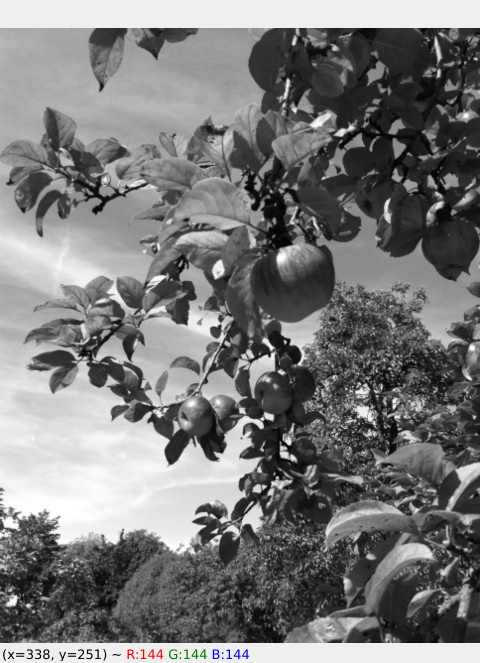
\includegraphics[width=0.6\textwidth, keepaspectratio]{gauss.png}\\
  3x3 Gauss-Filter ($\sigma = 0.5$)
\end{figure}

\newpage

\subsection*{b) Kanten finden}
Als zweiten Schritt soll aus dem geglätteten Bild jeweils in vertikaler und horizontaler Richtung ein Gradient errechnet werden, und aus diesen Gradienten der Betrag und die Richtung errechnet werden.
Dieses ist in der Funktion \textbf{detect\_edges} (main.py Zeile 34) implementiert, welche als Parameter das geglättete Bild \textbf{img} übergeben bekommt.
Die Funktion wendet zunächst einen Sobel-Filter auf das geglättete Bild an, hier werden für die x- und y-Richtung folgende Kernel verwendet:

\begin{equation*}
  Sobel_x =
  \begin{bmatrix}
    -1 & 0 & 1 \\
    -2 & 0 & 2 \\
    -1 & 0 & 1
  \end{bmatrix}
\end{equation*}
  
\begin{equation*}
  Sobel_y =
  \begin{bmatrix}
    -1 & -2 & -1 \\
     0 &  0 &  0 \\
     1 &  2 &  1
  \end{bmatrix}
\end{equation*}

Anschließend werden aus den resultierenden Gradienten für jeden Punkt der Betrag und die Richtung folgendermaßen berechnet:

\begin{equation*}
  |\Delta g| = \sqrt{g_x^2 + g_y^2}
\end{equation*}
\begin{equation*}
  \alpha(\Delta g) = \arctan{\frac{g_y}{g_x}}
\end{equation*}

\subsubsection*{Ergebnisbilder}
\begin{figure}[H]
  \centering
  \begin{minipage}{0.49\textwidth}
    \centering
    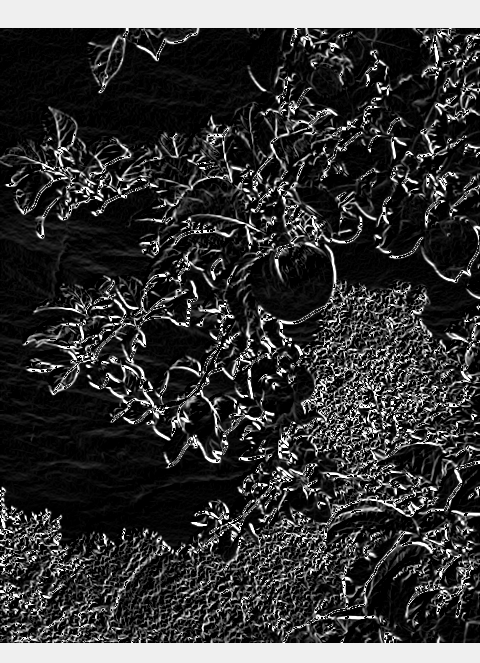
\includegraphics[width=\textwidth, height=0.4\textheight, keepaspectratio]{value.png}
    Gradientenbetrag
  \end{minipage}
  \begin{minipage}{0.49\textwidth}
    \centering
    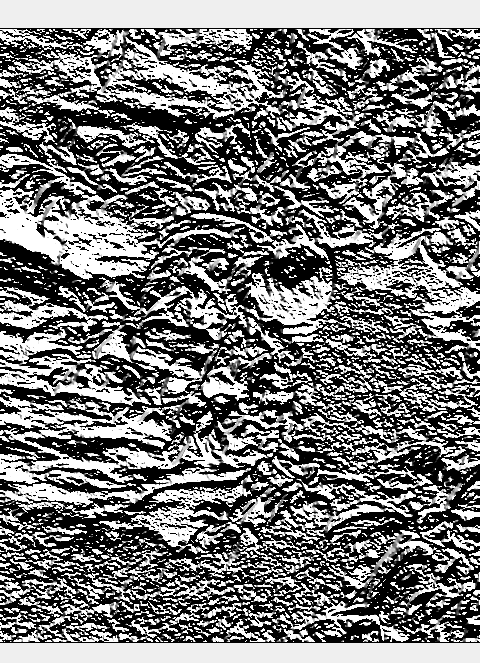
\includegraphics[width=\textwidth, height=0.4\textheight, keepaspectratio]{direction.png}
    Gradientenrichtung
  \end{minipage}
\end{figure}

\subsection*{c) Kanten ausdünnen (Non-maxima-suppression)}
Mithilfe des Gradientenbetrags und der Gradientenrichtung, soll im nöchsten Schritt eine Non-maxima-suppression durchgeführt werden.
Diese ist in der Funktion \textbf{suppress\_gradient} (main.py Zeile 59) implementiert.
Hierbei soll nur die Maxima des Gradienten übernommen, welche anhand der Gradientenrichtung bestimmt werden.

\subsubsection*{Ergebnisbild}
\begin{figure}[H]
  \centering
  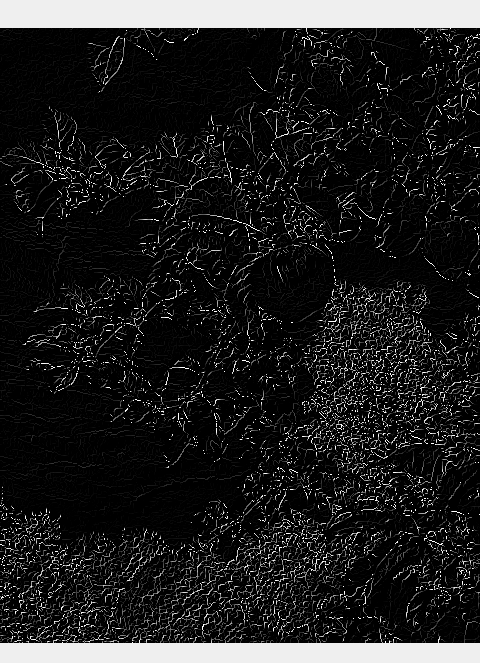
\includegraphics[width=0.6\textwidth, keepaspectratio]{suppressed.png}\\
  Non-maxima-suppression
\end{figure}

\newpage

\subsection*{d) Zusammengehörige Kanten finden (Hysterese)}
Der letzte Schritt des Canny-Kantendetektors ist eine Hysterese, welche in der Funktion \textbf{} (main.py Zeile 103) implementiert wurde.

\subsubsection*{Ergebnisbild}
\begin{figure}[H]
  \centering
  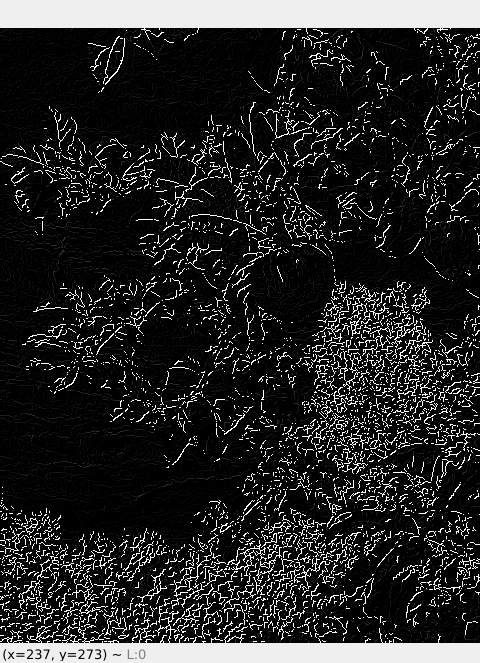
\includegraphics[width=0.6\textwidth, keepaspectratio]{hysteresis.png}\\
  Hysterese ($t_{low} = 50$, $t_{high} = 100$)
\end{figure}




\end{document}
